

\begin{figure}[]
\centering
\begin{subfigure}[b]{0.47\textwidth}
    \centering
    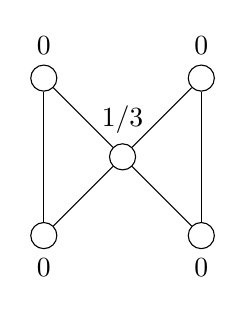
\begin{tikzpicture}
        \tikzstyle{vertex}=[circle, draw]
        \node[vertex, label=above:$1/3$](v) at (0, 0) {};
        \node[vertex, label=above:$0$](a) at (-1, 1) {};
        \node[vertex, label=above:$0$](b) at (1, 1) {};
        \node[vertex, label=below:$0$](c) at (-1,-1) {};
        \node[vertex, label=below:$0$](d) at (1,-1) {};
            \begin{scope}[every path/.style={-}, every node/.style={inner sep=1pt}]
                   \draw (a) -- (c);
                   \draw (b) -- (d);
                   \draw (a) -- (v);
                   \draw (b) -- (v);
                   \draw (c) -- (v);
                   \draw (d) -- (v);
            \end{scope} 
        \end{tikzpicture}
        \caption{The unique extreme point in the weak density polyhedron along the all-ones objective direction for the butterfly graph is as shown. The largest coordinate is $1/3$ and all other coordinates are $0$. Consequently, the integrality gap of the LP $\min\{\sum_{u\in V}x_u: x\in \weakdensitypolyhedron(G)\}$ is at least $3$.}
        \label{fig:butterfly-WD-integrality-gap}
     \end{subfigure}
     \hfill
     \begin{subfigure}[b]{0.47\textwidth}
    \centering
    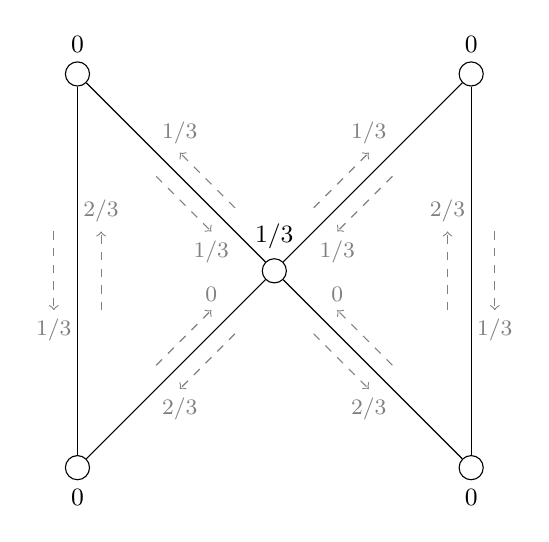
\begin{tikzpicture}
    \small
        \tikzstyle{vertex}=[circle, draw]
        \node[vertex, label=above:$1/3$](v) at (0, 0) {};
        \node[vertex, label=above:$0$](a) at (-2.5, 2.5) {};
        \node[vertex, label=above:$0$](b) at (2.5, 2.5) {};
        \node[vertex, label=below:$0$](c) at (-2.5,-2.5) {};
        \node[vertex, label=below:$0$](d) at (2.5,-2.5) {};
            % \begin{scope}[every path/.style={-}, every node/.style={inner sep=1pt}]
                    \draw (a) -- (c);
                   \draw (b) -- (d);
                   \draw (a) -- (v);
                   \draw (b) -- (v);
                   \draw (c) -- (v);
                   \draw (d) -- (v);
            % \end{scope} 

        \draw[->, gray, dashed] (-2.2, -0.5) to (-2.2, 0.5)  node[above] {\footnotesize $2/3$};
        \draw[->, gray, dashed] (-2.8, 0.5) to (-2.8, -0.5) node[below] {\footnotesize $1/3$};

        \draw[->, gray, dashed] (2.2, -0.5) to (2.2, 0.5) node[above] {\footnotesize $2/3$};
        \draw[->, gray, dashed] (2.8, 0.5) to (2.8, -0.5) node[below] {\footnotesize $1/3$};

        \draw[->, gray, dashed] (-1.5, -1.2) to (-0.8, -0.5) node[above] {\footnotesize $0$};
        \draw[->, gray, dashed] (-0.5, -0.8) to (-1.2, -1.5) node[below] {\footnotesize $2/3$};

        \draw[->, gray, dashed] (1.5, 1.2) to (0.8, 0.5) node[below] {\footnotesize $1/3$};
        \draw[->, gray, dashed] (0.5, 0.8) to (1.2, 1.5) node[above] {\footnotesize $1/3$};

        \draw[->, gray, dashed] (-1.5, 1.2) to (-0.8, 0.5) node[below] {\footnotesize $1/3$};
        \draw[->, gray, dashed] (-0.5, 0.8) to (-1.2, 1.5) node[above] {\footnotesize $1/3$};

        \draw[->, gray, dashed] (1.5, -1.2) to (0.8, -0.5) node[above] {\footnotesize $0$};
        \draw[->, gray, dashed] (0.5, -0.8) to (1.2, -1.5) node[below] {\footnotesize $2/3$};
        
        \end{tikzpicture}
        \caption{A minimal extreme point in the orientation polyhedron along the all-ones objective direction for the butterfly graph is as shown. The largest $x$-coordinate is $1/3$ and all other $x$-coordinates are $0$. Consequently, the integrality gap of the LP $\min\{\sum_{u\in V}x_u: x\in \orientationpolyhedron(G)\}$ is at least $3$.}
        \label{fig:butterfly-orientation-integrality-gap}
\end{subfigure}
     
\end{figure}